\documentclass{standalone}
\usepackage{tikz}

\begin{document}

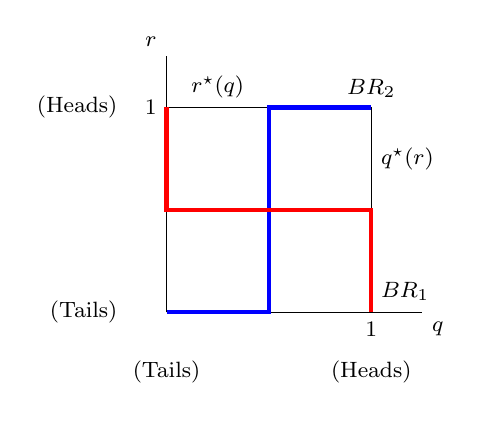
\begin{tikzpicture}[scale=0.65,font=\footnotesize]
\draw (0,0)--(5,0) node[pos=.8, below]{1} node[below right]{$q$};
\draw (0,0)--(0,5) node[pos=.8, left]{1} node[above left]{$r$};
\draw (0,4)-|(4,0) node[pos=0.125, above] {$r^\star(q)$} node[pos=0.500,above]{$BR_{2}$} node[pos=0.625,right]{$q^\star(r)$} node[pos=0.950,right]{$BR_{1}$};
\draw[ultra thick, blue] (0,0)--(2,0)|-(4,4);
\draw[ultra thick, red] (0,4)--(0,2)-|(4,0);
\node[below=5mm] at (0,0){(Tails)};
\node[below=5mm] at (4,0){(Heads)};
\node[left=5mm] at (0,0){(Tails)};
\node[left=5mm] at (0,4){(Heads)};
\end{tikzpicture}

\end{document}
